\documentclass[a4paper,12pt,english]{article}
\usepackage{glossaries}
\usepackage[T1]{fontenc}
\usepackage{babel}
\usepackage{graphicx}
\usepackage[table,xcdraw]{xcolor}
\usepackage{hyperref}
\usepackage{blindtext}
\usepackage{geometry}
\usepackage{parskip}
\usepackage{mathtools}
\usepackage{siunitx}
\usepackage{listings}
\usepackage{csquotes}
\usepackage{caption}
\usepackage{subcaption}
\usepackage{comment}
\usepackage{pdfpages}
\usepackage{pict2e}

% \DeclareRobustCommand{\slashcirc}{{\mathpalette\doslashcirc\relax}}

% \makeatletter
% \newcommand\doslashcirc[2]{%
%   \sbox\z@{$#1\m@th\circ$}%
%   \setlength\unitlength{\wd\z@}
%   \begin{picture}(1,1)
%   \roundcap
%   \put(0,0){\box\z@}
%   \put(0,0){\line(1,1){1}}
%   \end{picture}%
% }
% \makeatother


% %% Some packages you will need
% \usepackage{pgfplots}
% \usepackage{pgfplotstable}
% \usepackage{booktabs}
% \usepackage{array}
% \usepackage{colortbl}


\definecolor{arduinoorange}{HTML}{FFA500}
\definecolor{arduinogray}{HTML}{808080}
\definecolor{arduinoblue}{HTML}{007ACC}
\definecolor{arduinogreen}{HTML}{469B00}

\lstset{
  language=C++,
  basicstyle=\ttfamily\footnotesize,
  keywordstyle=\color{arduinoorange},
  stringstyle=\color{arduinogreen},
  commentstyle=\color{arduinogray},
  moredelim=[s][\color{arduinoblue}]{\#}{\ },
  morekeywords={digitalRead,digitalWrite,pinMode,analogRead,analogWrite,Serial,begin,HIGH,LOW},
  frame=tb,
  tabsize=4,
  showstringspaces=false,
  breaklines=true,
  numbers=left,
  numberstyle=\tiny\color{arduinogray},
  numbersep=5pt,
  extendedchars=true,
  literate={á}{{\'a}}1 {ã}{{\~a}}1 {é}{{\'e}}1,
}

\lstdefinestyle{Arduino}
{
  language=C++,
  basicstyle=\ttfamily\footnotesize,
  keywordstyle=\color{arduinoorange},
  stringstyle=\color{arduinogreen},
  commentstyle=\color{arduinogray},
  moredelim=[s][\color{arduinoblue}]{\#}{\ },
  morekeywords={digitalRead,digitalWrite,pinMode,analogRead,analogWrite,Serial,begin},
  frame=tb,
  tabsize=4,
  showstringspaces=false,
  breaklines=true,
  numbers=left,
  numberstyle=\tiny\color{arduinogray},
  numbersep=5pt,
  extendedchars=true,
  literate={á}{{\'a}}1 {ã}{{\~a}}1 {é}{{\'e}}1,
  backgroundcolor=\color{black!85},
  rulecolor=\color{arduinoorange},
  frame=single,
  frameround=tttt,
  framexleftmargin=6pt,
  framexrightmargin=6pt,
  framextopmargin=6pt,
  framexbottommargin=6pt,
  breaklines=true,
  postbreak=\raisebox{0ex}[0ex][0ex]{\ensuremath{\color{red}\hookrightarrow\space}},
}

\usepackage[
    backend=biber,
    backref=true,
    backrefstyle=none,
    sortcites=true,
    sorting=none,
    doi=false, % doi informatie wordt niet weergegeven
    %uniquename=true,
    %uniquelist=true,
    maxcitenames=3,
    %issn=false, werkt niet
    language=american
]{biblatex}
\addbibresource{information/Sources.bib}
\DefineBibliographyStrings{english}{
    backrefpage = {blz.},
    backrefpages = {blz.},
}
\makeglossaries
\definecolor{Grey1}{HTML}{343434}
\graphicspath{{./Media/Figuren/}}
 \geometry{
 a4paper,
 total={170mm,257mm},
 left=20mm,
 top=20mm,
 }
\hypersetup{
    colorlinks=true,
    linkcolor=blue,
    filecolor=magenta,      
    urlcolor=cyan,
    pdftitle={Overleaf Example},
    pdfpagemode=FullScreen,
    }


\begin{document}
\title{

\includegraphics[width=3.5in]{img/Logo.png} \\
\vspace*{1in}
\textbf{ELOMVO}\\
\textit{Prakticum}\\
Version 1
}
\author{
\vspace*{0.5in} \\
  Written by:\\
  Laurens van der Drift\\
\vspace*{0.2in} \\
    The Hague University of Applied Sciences\\
    \textbf{Electrical Engineering}\\
    Delft, The Netherlands
   } 
\maketitle
\newpage
\tableofcontents
\section{CASPOC Simulaties Boost}
\subsection{Inleiding en doel boostconverter}
\subsection{Simulatie}
\subsection{CASPOC Simulaties Buck-converter}
\subsubsection{Verschillende duty cycles}
\subsection{Continubedrijf en dutycycle}
\subsection{Inductieve belasting}
\subsection{Vermogen}
\subsection{Stroomwet van Kirchhof}
\subsection{Snelheid van de responsie}
\subsection{Conclusie}

\subsection{Simulatie}
\begin{figure}[h!]
    \centering
    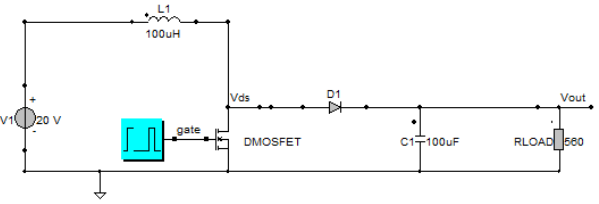
\includegraphics[width=1\linewidth]{img/hfd1/Schema voor de simulatie van een boostconverter.png}
    \caption{Schema voor de simulatie van een boostconverter}
    \label{fig:Schema voor de simulatie van een boostconverter}
\end{figure}
\begin{table}[h!]
\centering
\begin{tabular}{|l|c|c|c|}
\hline
\textbf{Duty Cycle (\%)} & \textbf{Vuit (V) Rl=1MEG (onbelast)} & \textbf{Vuit (V) Rl=560 Ohm} & \textbf{Vuit (V) Rl=56 Ohm} \\ \hline
10 & 42.77 & 42.57 & 41.98 \\ \hline
20 & 48.41 & 48.01 & 47.26 \\ \hline
40 & 65.02 & 64.34 & 62.91 \\ \hline
50 & 77.95 & 77.23 & 75.25 \\ \hline
75 & 139.54 & 138.83 & 132.72 \\ \hline
\end{tabular}
\caption{Uitgangsspanningen Vuit bij verschillende belasting en duty cycles}
\end{table}
Uit de simulaties blijkt dat de uitgangsspanning toeneemt met een hogere duty cycle, zoals verwacht bij een boostconverter. De belasting beïnvloedt de spanning: bij zwaardere belasting daalt de uitgangsspanning licht. De resultaten komen goed overeen met de theorie en tonen de correcte werking van de schakeling. De wet van Kirchhoff en \(UL = L \cdot \frac{dI}{dt}\) zijn duidelijk waarneembaar in de stroom- en spanningsgolfvormen.

\subsubsection{10\% dutycycle, 1 MEG ohm load}
\begin{figure}[h!]
    \centering
    \begin{subfigure}[b]{0.3\linewidth}
        \centering
        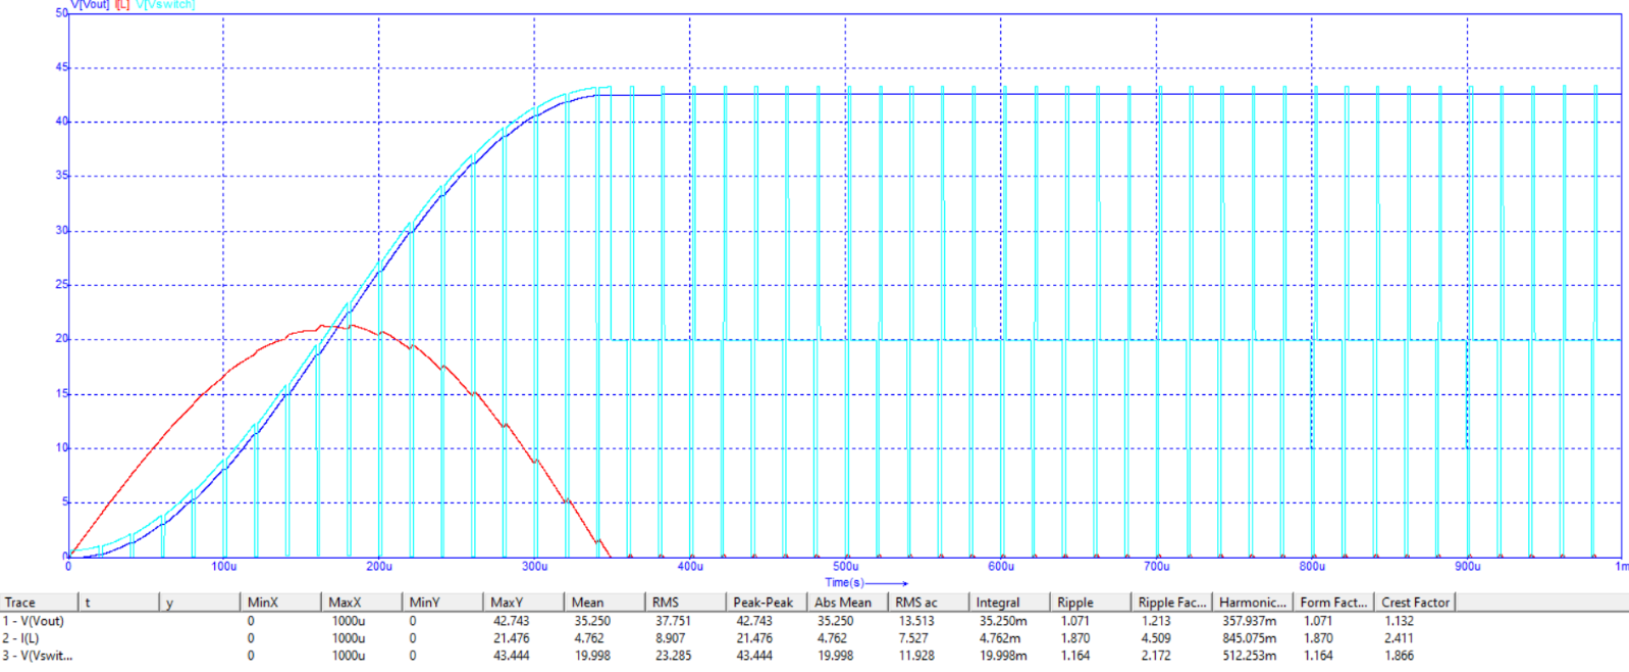
\includegraphics[width=\linewidth]{img/hfd1/hfd1-10pduty-1MEG-INDUCTOR.png}
        \caption{Spoelstroom}
        \label{fig:inductor}
    \end{subfigure}
    \hfill
    \begin{subfigure}[b]{0.3\linewidth}
        \centering
        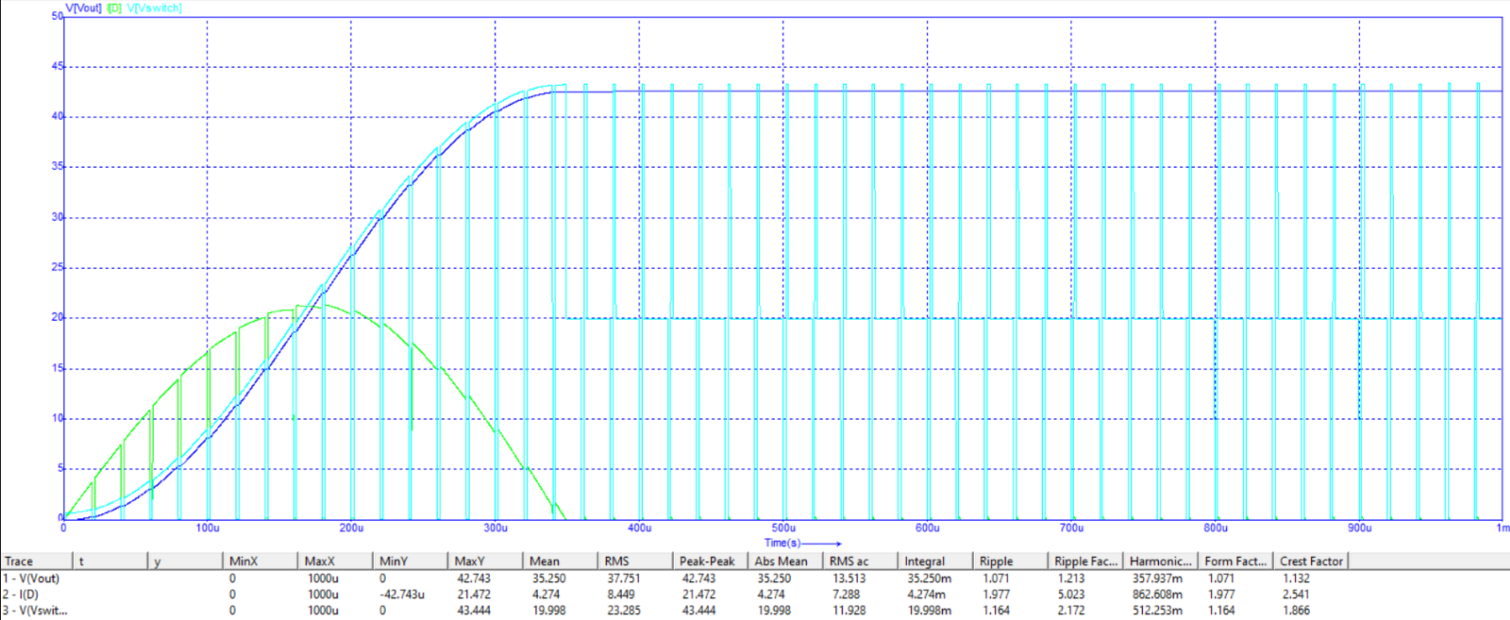
\includegraphics[width=\linewidth]{img/hfd1/hfd1-10pduty-1MEG-DIODE.png}
        \caption{Diodestroom}
        \label{fig:diode}
    \end{subfigure}
    \hfill
    \begin{subfigure}[b]{0.3\linewidth}
        \centering
        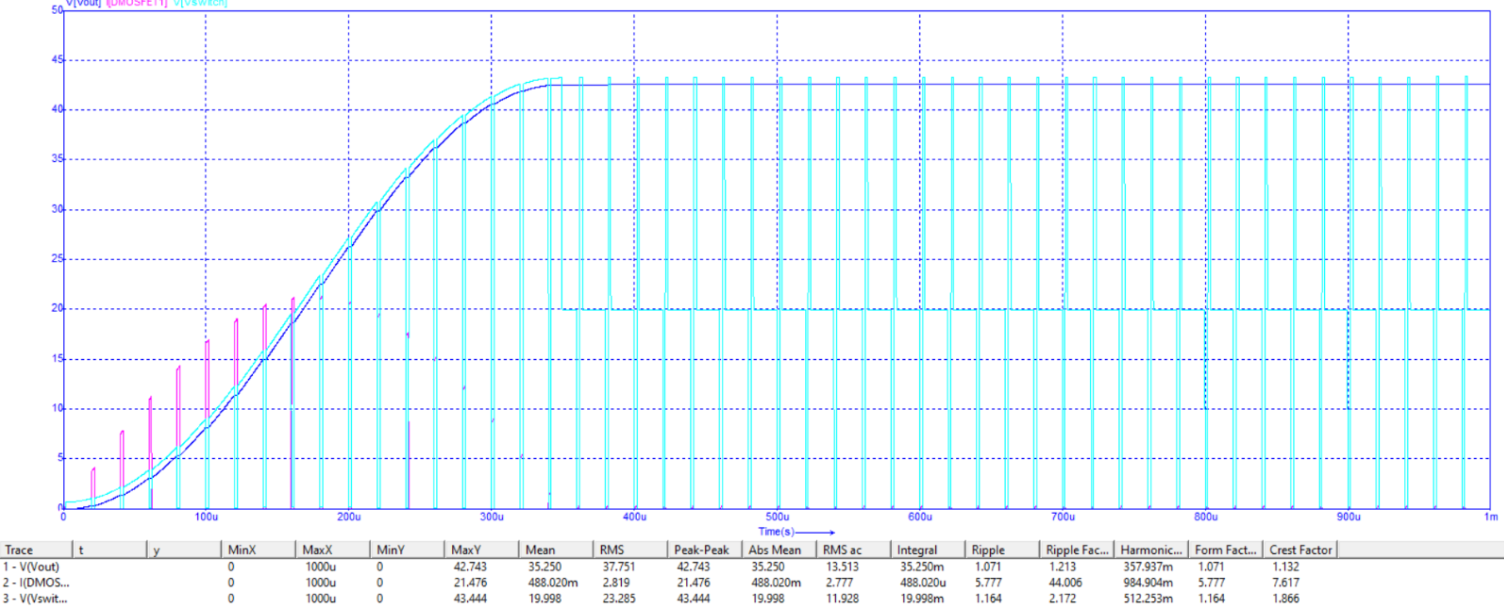
\includegraphics[width=\linewidth]{img/hfd1/hfd1-10pduty-1MEG-DMOSFET.png}
        \caption{Mosfetstroom}
        \label{fig:mosfet}
    \end{subfigure}
    
    \caption{Vergelijking van stroom en spanning bij verschillende componenten met een weerstand van 1M\(\Omega\) en duty cycle van 10\%.}
    \label{fig:componenten}
\end{figure}




\subsubsection{40\% duty cycle, 560 ohm load}
\begin{figure}[h!]
    \centering
    \begin{subfigure}[b]{0.3\linewidth}
        \centering
        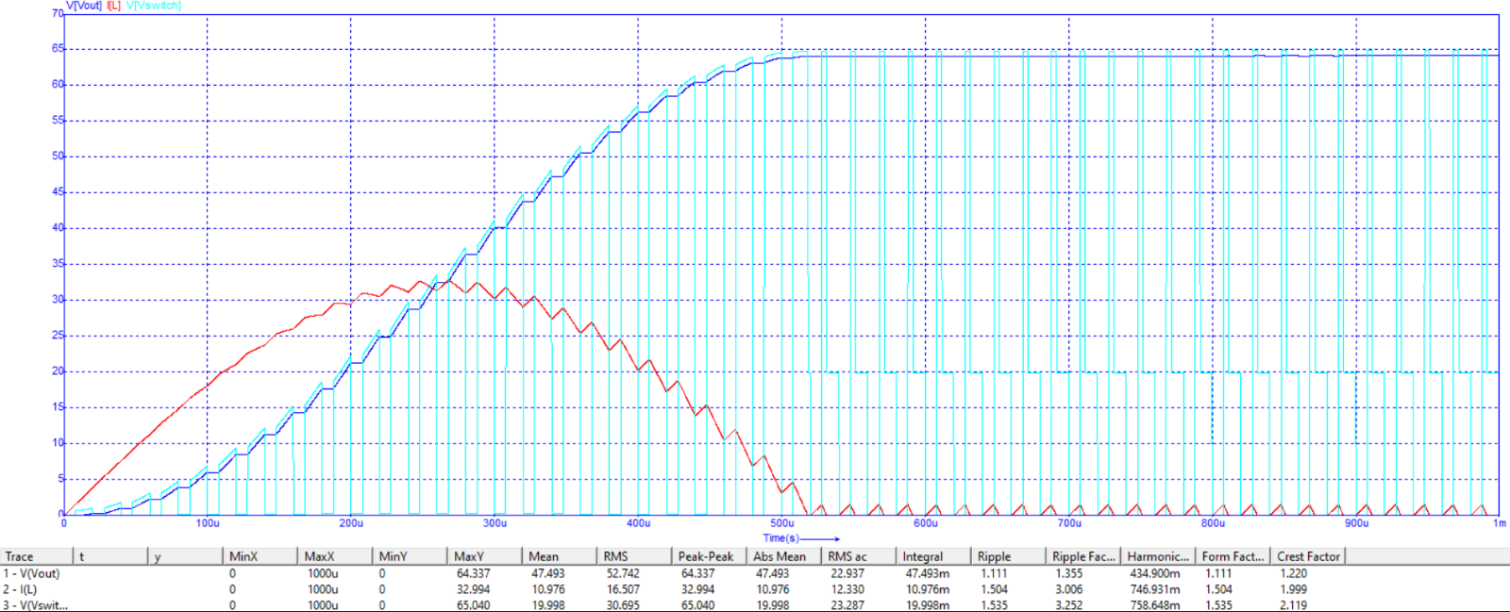
\includegraphics[width=\linewidth]{img/hfd1/hfd1-40pduty-560-INDUCTOR.png}
        \caption{Spoelstroom}
        \label{fig:inductor40}
    \end{subfigure}
    \hfill
    \begin{subfigure}[b]{0.3\linewidth}
        \centering
        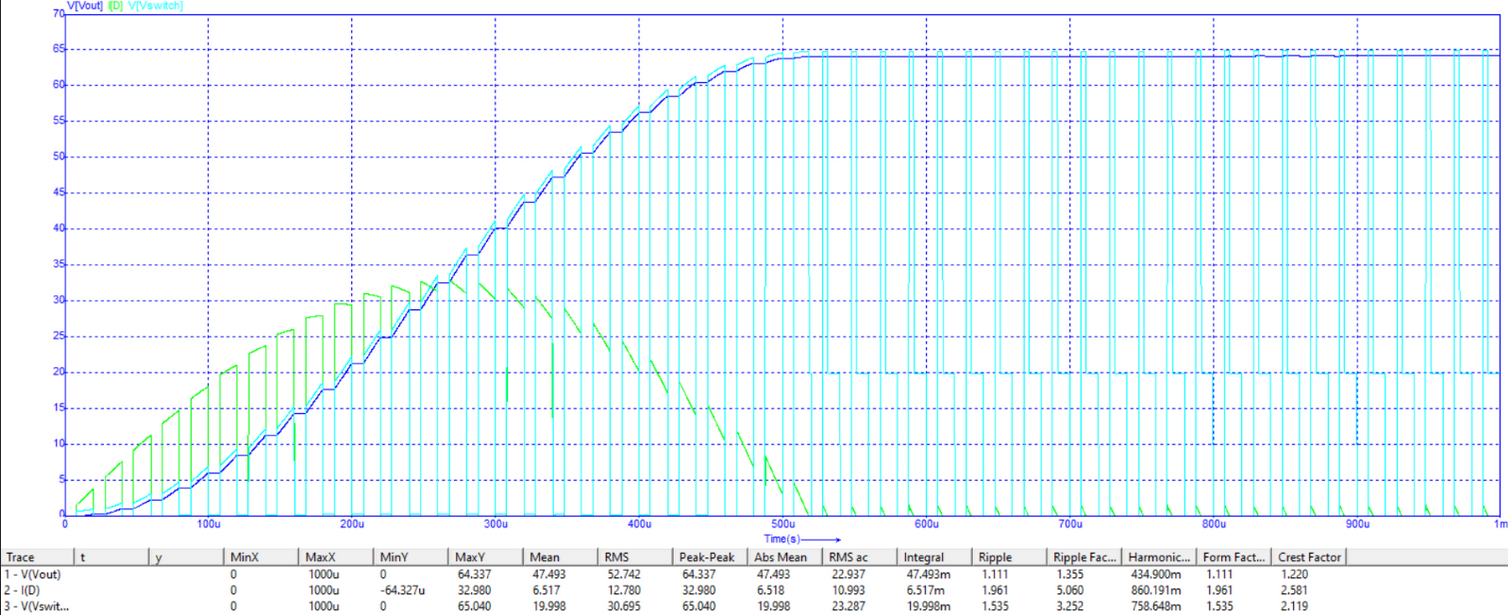
\includegraphics[width=\linewidth]{img/hfd1/hfd1-40pduty-560-DIODE.png}
        \caption{Diodestroom}
        \label{fig:diode40}
    \end{subfigure}
    \hfill
    \begin{subfigure}[b]{0.3\linewidth}
        \centering
        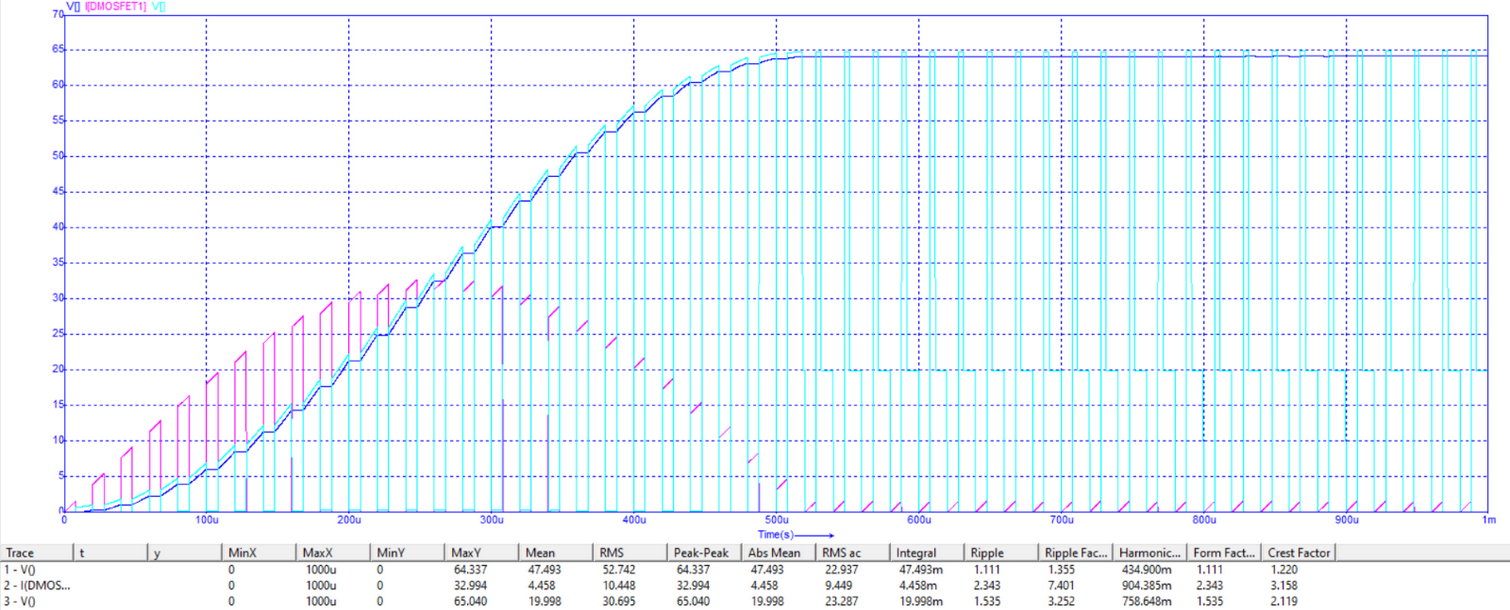
\includegraphics[width=\linewidth]{img/hfd1/hfd1-40pduty-560-MOSFET.png}
        \caption{Mosfetstroom}
        \label{fig:mosfet40}
    \end{subfigure}
    
    \caption{Vergelijking van stroom en spanning bij verschillende componenten met een weerstand van 560\(\Omega\) en duty cycle van 40\%.}
    \label{fig:componenten40}
\end{figure}




\subsubsection{75\% duty cycle, 56 ohm load}

\begin{figure}[h!]
    \centering
    \begin{subfigure}[b]{0.3\linewidth}
        \centering
        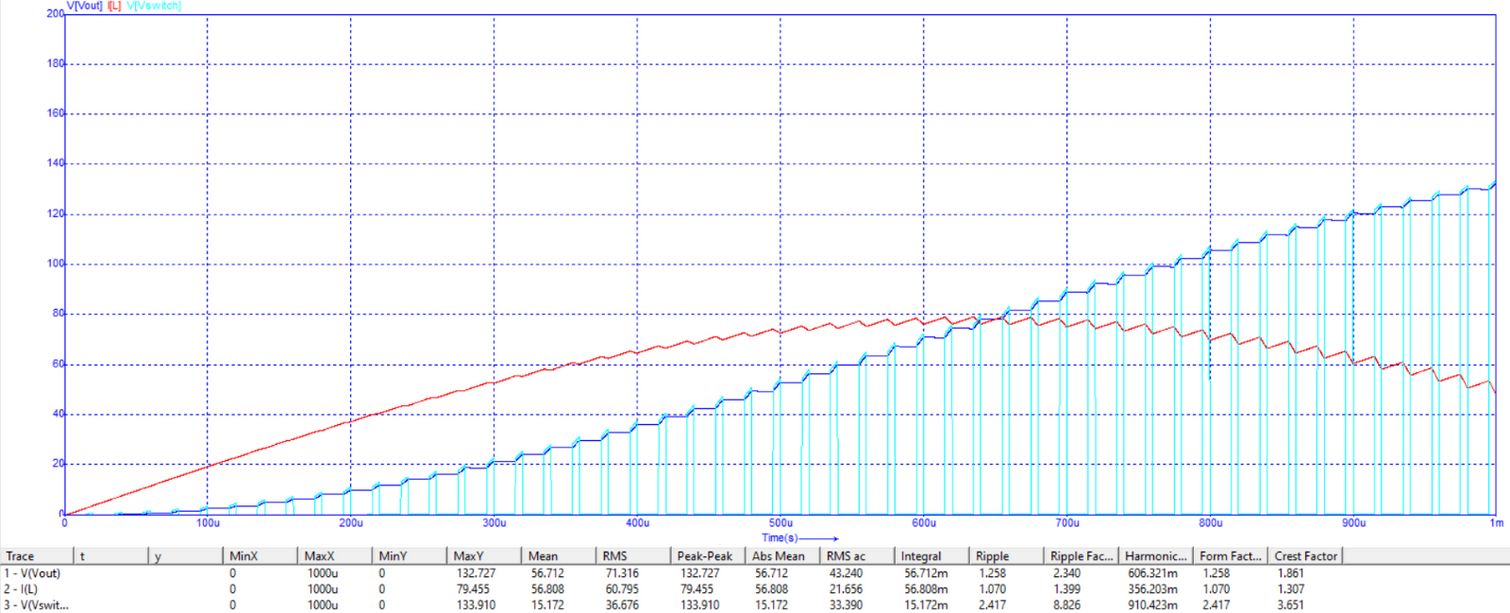
\includegraphics[width=\linewidth]{img/hfd1/hfd1-75pduty-56-INDUCTOR.png}
        \caption{Spoelstroom}
        \label{fig:inductor75}
    \end{subfigure}
    \hfill
    \begin{subfigure}[b]{0.3\linewidth}
        \centering
        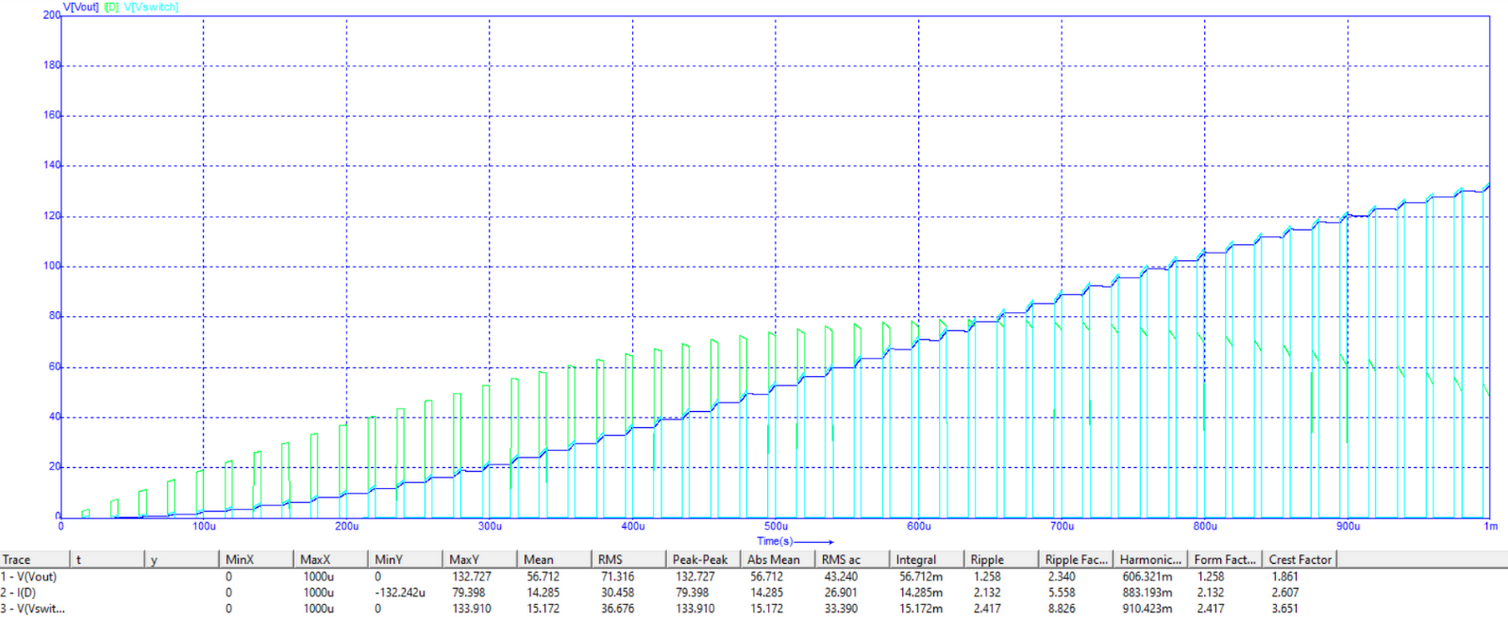
\includegraphics[width=\linewidth]{img/hfd1/hfd1-75pduty-56-DIODE.png}
        \caption{Diodestroom}
        \label{fig:diode75}
    \end{subfigure}
    \hfill
    \begin{subfigure}[b]{0.3\linewidth}
        \centering
        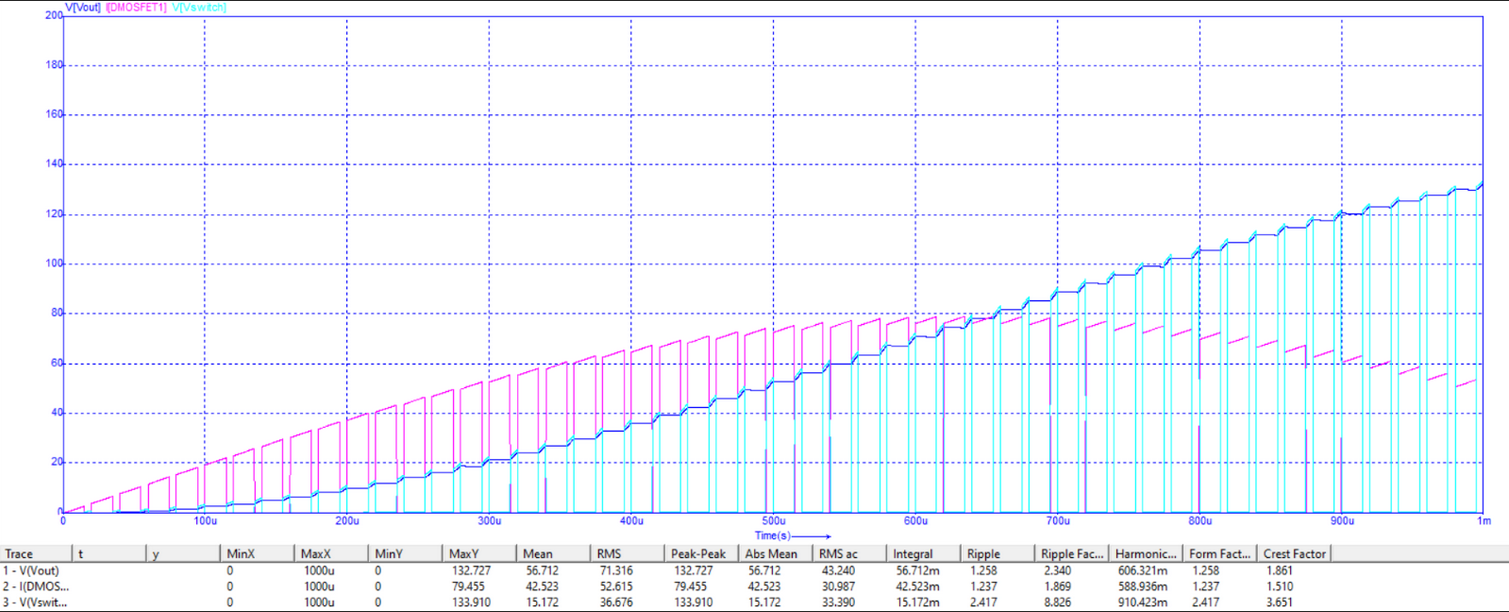
\includegraphics[width=\linewidth]{img/hfd1/hfd1-75pduty-56-DMOSFET.png}
        \caption{Mosfetstroom}
        \label{fig:mosfet75}
    \end{subfigure}
    
    \caption{Vergelijking van stroom en spanning bij verschillende componenten met een weerstand van 56\(\Omega\) en duty cycle van 75\%.}
    \label{fig:componenten75}
\end{figure}

[HIER MOET NOG UITLEG KOMEN]
\subsection{CASPOC Simulaties Buck-converter}
\subsubsection{Verschillende duty cycles}

\subsection{Continubedrijf en dutycycle}

\subsection{Inductieve belasting}

\subsection{Vermogen}
\textcolor{gray}{Meet de gemiddelde ingangsstroom}\newline
Gemiddelde Ingangsstroom, \(I_{in, gem}\) = -0,623A , \(V_{in}\) = 20V , \(P_{in}\) = 12,46W \newline

\textcolor{gray}{Meet de gemiddelde uitgangsstroom}\newline
Gemiddelde Uitgangsstroom, \(I_{uit, gem}\) = -1,008A , \(V_{in}\) =  10,08V , \(P_{in}\) = 10,16W

\textcolor{gray}{Is het ingangsvermogen gelijk aan het uitgangsvermogen?}\newline
Het ingangs- en uitgangsvermogen zijn niet gelijk aan elkaar. Bij een ideale converter zou dit wel het geval zijn. In een echte buck converter zijn er echter kleine verliezen door weerstand in de spoel, het schakelen, en verliezen in de MOSFET en diode. Deze verliezen zorgen ervoor dat \(P_{in}\) iets groter is dan \(P_{uit}\).  
\subsection{Stroomwet van Kirchhof}
\textcolor{gray}{Meet de gemiddelde stroom door de spoel L}\newline
Gemiddelde spoel door de stroom, \(I_{L_{gem}}\) = 1,201A \newline
\newline
\textcolor{gray}{Meet de gemiddelde stroom door de Mosfet}\newline
Gemiddelde spoel door de MOSFET, \(I_{MOSFET_{gem}}\) = 0,623A\newline
\newline
\textcolor{gray}{Meet de gemiddelde stroom door de diode}\newline
Gemiddelde spoel door de Diode, \(I_{D_{gem}}\) = 0,534A\newline
\newline
\textcolor{gray}{Had je deze waarden ook uit de gemeten in en uitgangsstroom kunnen bepalen?}\newline
Nee deze waardes zijn niet te bepalen met de gemeten in en uitgangsstroom.


\subsection{Snelheid van de responsie}

\textcolor{gray}{Meet de maximale peak van de spoelstroom en de minimale peak} \newline
Maximale spoelstroom, \(I_{L_{MAX}}\) = 1,377A \newline
Minimale spoelstroom, \(I_{L_{MIN}}\) = 0,551A\newline

\textcolor{gray}{Meet de tijd die nodig is voor de spoelstroom om van de minimale waarde naar de maximale
waarde te gaan.} \newline
De tijd om van minimale peak naar maximale peak te komen is 0,01 us \newline
\newline
\textcolor{gray}{Kan je uit deze drie meetgegevens di/dt afleiden?} \newline
Ja, dat kan. Door de verandering in spoelstroom te delen door de tijd van de peak-to-peak. \newline

\textcolor{gray}{Kan je de waarde van de spoel berekenen met behulp van de gemeten di/dt en de in- en
uitgangsspanningen van de buck converter? Is dit dan de waarde van 100uH?}komen de berekeningen uit op 125\(\mu\)H dus niet 100\(\mu\)H. Dit komt doordat de bij \autoref{sub:1.5_ind_bel} gekozen spoelwaarde (125\(\mu\)H) aangehouden is, dus komt de berekening wel uit op de juiste spoelwaarde. 

\subsection{Conclusie}

Uit de simulaties bleek dat de boostconverter goed functioneerde zoals verwacht. Er was een duidelijke relatie tussen de duty cycle, de belasting en de uitgangsspanning. Dit toont de relatie van de converter aan met verschillende component waarden.

\section{Online Simulatie Buck}
\subsection{Buck converter}
Er zijn een aantal componentwaarden gegeven die we hebben ingevoerd in het simulatiecircuit. Deze waarden zijn weergegeven in \autoref{fig:Gegeven Componentwaarden}.
\begin{table}[h!]
\centering
\begin{tabular}{|l|l|}
\hline
\textbf{Component} & \textbf{Value} \\
\hline
Vin & 48 volt \\
L   & 220 $\mu$H \\
C   & 10 $\mu$F \\
Rout & 10 \\
Fs  & 50 kHz \\
d   & 25\% \\
\hline
\end{tabular}
\caption{Gegeven Componentwaarden}\label{fig:Gegeven Componentwaarden}
\end{table}
In de opdracht wordt aangegeven dat we deze componentwaarden moeten gebruiken om met verschillende waarden voor de duty cycle (D) te simuleren. De resultaten van deze simulaties zijn weergegeven in \autoref{fig:Overzicht van meetwaarden variabele duty cycle}
\begin{table}[h!]
\centering
\begin{tabular}{|c|c|c|c|c|c|c|c|}
\hline
\textbf{D} & \textbf{Vin} & \textbf{Iin} & \textbf{Vout} & \textbf{Iout} & \textbf{Pin} & \textbf{Pout} & \textbf{n} \\
\hline
10 & 48 & 0,559144 & 4,72 & 0,47204 & 26,838912 & 2,2280288 & 8,30\% \\
20 & 48 & 1,163 & 9,482 & 0,948209 & 55,824 & 8,990917738 & 16,11\% \\
30 & 48 & 1,807 & 14,191 & 1,419 & 86,736 & 20,137029 & 23,22\% \\
40 & 48 & 2,272 & 19,037 & 1,904 & 109,056 & 36,246448 & 33,24\% \\
50 & 48 & 2,365 & 23,625 & 2,362 & 113,52 & 55,80225 & 49,16\% \\
60 & 48 & 3,202 & 28,474 & 2,847 & 153,696 & 81,065478 & 52,74\% \\
70 & 48 & 3,355 & 33,314 & 3,331 & 161,04 & 110,968934 & 68,91\% \\
80 & 48 & 4,117 & 38,087 & 3,809 & 197,616 & 145,073383 & 73,41\% \\
90 & 48 & 4,463 & 43,001 & 4,3 & 214,224 & 184,9043 & 86,31\% \\
\hline
\end{tabular}
\caption{Overzicht van meetwaarden variabele duty cycle}\label{fig:Overzicht van meetwaarden variabele duty cycle}
\end{table}
Daarna wordt ons gevraagd om de waarden van Rout aan te passen. De resultaten voor de efficiëntie ($\eta$) bij verschillende waarden van Rout zijn weergegeven in \autoref{fig:Overzicht van meetwaarden bij verschillende Rout waarden}.
\begin{table}[h!]
\centering
\begin{tabular}{|c|c|c|c|c|c|c|c|}
\hline
\textbf{Rout} & \textbf{Vin} & \textbf{Iin} & \textbf{Vout} & \textbf{Iout} & \textbf{Pin} & \textbf{Pout} & \textbf{n} \\
\hline
2  & 48 & 6,011   & 11,8  & 5,9     & 288,528  & 69,62     & 24,13\% \\
4  & 48 & 3,245   & 11,817 & 2,954   & 155,76   & 34,907418 & 22,41\% \\
6  & 48 & 2,119   & 11,873 & 1,979   & 101,712  & 23,496667 & 23,10\% \\
8  & 48 & 1,632   & 11,901 & 1,488   & 78,336   & 17,708688 & 22,61\% \\
10 & 48 & 1,483   & 11,864 & 1,186   & 71,184   & 14,070704 & 19,77\% \\
12 & 48 & 1,286   & 11,866 & 0,999827 & 61,728   & 11,86394718 & 19,22\% \\
14 & 48 & 1,145   & 11,87  & 0,847829 & 54,96    & 10,06373023 & 18,31\% \\
16 & 48 & 1,039   & 11,875 & 0,742163 & 49,872   & 8,813185625 & 17,67\% \\
18 & 48 & 0,955579 & 11,875 & 0,659737 & 45,867792 & 7,834376875 & 17,08\% \\
20 & 48 & 0,74917  & 11,934 & 0,596704 & 35,96016  & 7,121065536 & 19,80\% \\
\hline
\end{tabular}
\caption{Overzicht van meetwaarden bij verschillende Rout waarden}\label{fig:Overzicht van meetwaarden bij verschillende Rout waarden}
\end{table}
\subsection{Inductor current ripple}
Voor de volgende opdracht krijgen wij een aantal waardes(\autoref{fig:Componentwaarden voor simulatie2.1}) gegeven, waarna we de waarde van de spoel zullen variëren om de effecten te observeren.
\begin{table}[h!]
\centering
\begin{tabular}{|l|l|}
\hline
\textbf{Component} & \textbf{Value} \\
\hline
Vin  & 48 volt \\
L    & 100 $\mu$H \\
C    & 10 $\mu$F \\
Rout & 10 \\
Fs   & 50 kHz \\
d    & 40\% \\
\hline
\end{tabular}
\caption{Componentwaarden voor simulatie}
\label{fig:Componentwaarden voor simulatie2.1}
\end{table}
De simulatie resulteert in de volgende waarden, zoals te zien in \autoref{fig:Inductor Current Ripple Waarden}
\begin{table}[h!]
\centering
\begin{tabular}{|l|c|c|c|}
\hline
\textbf{Inductor [H]} & \textbf{Current ripple [A]} & \textbf{MIN [A]} & \textbf{MAX [A]} \\
\hline
47u  & 2,948  & 0     & 2,948 \\
100u & 1,48   & 0,561 & 2,041 \\
150u & 1,577  & 0,056 & 1,633 \\
220u & 0,871  & 0,7   & 1,571 \\
470u & 0,313  & 1,053 & 1,366 \\
\hline
\end{tabular}
\caption{Inductor Current Ripple Waarden}
\label{fig:Inductor Current Ripple Waarden}
\end{table}
Dit herhalen we vervolgens, maar we veranderen de frequentie van 50 kHz naar 100 kHz. De resultaten zijn te zien in \autoref{fig:Inductor Current Ripple Waarden2}
\begin{table}[h!]
\centering
\begin{tabular}{|l|c|c|c|}
\hline
\textbf{Inductor [H]} & \textbf{Current ripple [A]} & \textbf{MIN [A]} & \textbf{MAX [A]}\\
\hline
47u  & 0,893067  & 0,716933  & 1,61 \\
100u & 0,892986  & 0,717014  & 1,61 \\
150u & 0,597264  & 0,869736  & 1,467 \\
220u & 0,28694   & 0,97206   & 1,259 \\
470u & 0,189     & 1,085     & 1,274 \\
\hline
\end{tabular}
\caption{Inductor Current Ripple Waarden}
\label{fig:Inductor Current Ripple Waarden2}
\end{table}
\subsection{Output voltage ripple}
\begin{table}[h!]
\centering
\begin{tabular}{|l|l|}
\hline
\textbf{Component} & \textbf{Value} \\
\hline
Vin  & 48 volt \\
L    & 100 $\mu$H \\
C    & 10 $\mu$F \\
Rout & 10 \\
Fs   & 50 kHz \\
d    & 40\% \\
\hline
\end{tabular}
\caption{Parameters for Output Voltage Ripple Simulation}
\label{fig:Output_voltage_ripple_simulation}
\end{table}
Als we deze gegevens invullen in de simulatie krijgen we de volgende resultaten te zien in \autoref{fig:Capacitor_voltage_ripple_waarden}
\begin{table}[h!]
\centering
\begin{tabular}{|l|c|c|c|}
\hline
\textbf{Capacitor} & \textbf{Voltage ripple} & \textbf{MIN} & \textbf{MAX} \\
\hline
10u   & 0,392 & 18,852 & 19,244 \\
22u   & 0,261 & 18,859 & 19,12  \\
47u   & 0,409 & 18,793 & 19,202 \\
100u  & 0,6   & 18,638 & 19,238 \\
220u  & 0,697 & 18,67  & 19,367 \\
470u  & 0,464 & 18,783 & 19,247 \\
\hline
\end{tabular}
\caption{Capacitor Voltage Ripple Waarden}
\label{fig:Capacitor_voltage_ripple_waarden}
\end{table}

Dit herhalen we vervolgens, maar we veranderen de frequentie van 50 kHz naar 100 kHz. De resultaten zijn te zien in \autoref{fig:Capacitor_voltage_ripple_waarden_100kHz}
\begin{table}[h!]
\centering
\begin{tabular}{|l|c|c|c|}
\hline
\textbf{Capacitor} & \textbf{Voltage ripple} & \textbf{MIN} & \textbf{MAX} \\
\hline
10u   & 0,087 & 18,962 & 19,049 \\
22u   & 0,012 & 18,995 & 19,007 \\
47u   & 0,269 & 18,88  & 19,149 \\
100u  & 0,299 & 18,858 & 19,157 \\
220u  & 1,018 & 18,434 & 19,452 \\
470u  & 0,699 & 18,609 & 19,308 \\
\hline
\end{tabular}
\caption{Capacitor Voltage Ripple Waarden bij 100 kHz}
\label{fig:Capacitor_voltage_ripple_waarden_100kHz}
\end{table}
\subsection{Output capacitor ESR}
In deze opdracht onderzoeken we de afhankelijkheid van de "output voltage ripple" van de equivalente seriesweerstand (Resr) van de condensator. We meten de piek-piek output voltage ripple bij verschillende Resr-waarden. De parameters voor de simulatie zijn als volgt:
\begin{table}[h!]
\centering
\begin{tabular}{|l|l|}
\hline
\textbf{Component} & \textbf{Value} \\
\hline
Vin  & 48 volt \\
L    & 100 $\mu$H \\
C    & 10 $\mu$F \\
Resr & 100 m$\Omega$ \\
Rout & 10 \\
Fs   & 50 kHz \\
d    & 40\% \\
\hline
\end{tabular}
\caption{Componentwaarden voor simulatie van de output voltage ripple}
\label{fig:Componentwaarden voor simulatie2.4}
\end{table}

De resultaten van de simulatie, waarin de Resr-waarde varieert, zijn te zien in \autoref{fig:Resr_Output_Voltage_Ripple_Waarden}.
\begin{table}[h!]
\centering
\begin{tabular}{|l|c|c|c|}
\hline
\textbf{Resr [\(\Omega\)]} & \textbf{Output voltage ripple [V]} & \textbf{MIN [V]} & \textbf{MAX [V]} \\
\hline
0,001  & 0,621  & 18,663  & 19,284 \\
0,01   & 0,583  & 18,713  & 19,296 \\
0,1    & 0,568  & 18,667  & 19,235 \\
0,2    & 0,578  & 18,703  & 19,281 \\
0,5    & 0,61   & 18,683  & 19,293 \\
1      & 0,562  & 18,667  & 19,229 \\
\hline
\end{tabular}
\caption{Output Voltage Ripple afhankelijk van Resr}
\label{fig:Resr_Output_Voltage_Ripple_Waarden}
\end{table}

Vervolgens verhogen we de frequentie van 50 kHz naar 100 kHz. De resultaten van deze simulatie zijn weergegeven in \autoref{fig:Resr_Output_Voltage_Ripple_Waarden_100kHz}.
\begin{table}[h!]
\centering
\begin{tabular}{|l|c|c|c|}
\hline
\textbf{Resr [\(\Omega\)]} & \textbf{Output voltage ripple [V]} & \textbf{MIN [V]} & \textbf{MAX [V]} \\
\hline
0,001  & 0,621  & 18,663  & 19,284 \\
0,01   & 0,583  & 18,713  & 19,296 \\
0,1    & 0,568  & 18,667  & 19,235 \\
0,2    & 0,578  & 18,703  & 19,281 \\
0,5    & 0,61   & 18,683  & 19,293 \\
1      & 0,562  & 18,667  & 19,229 \\
\hline
\end{tabular}
\caption{Output Voltage Ripple afhankelijk van Resr bij 100 kHz}
\label{fig:Resr_Output_Voltage_Ripple_Waarden_100kHz}
\end{table}
\subsection{Output capacitor ESR reduction}
In deze simulatie onderzoeken we de vermindering van de output voltage ripple door twee output condensatoren parallel te schakelen. De parameters van de simulatie zijn als volgt:
\begin{table}[h!]
\centering
\begin{tabular}{|l|l|}
\hline
\textbf{Component} & \textbf{Value} \\
\hline
Vin  & 48 volt \\
L    & 100 $\mu$H \\
C(2*) & 10 $\mu$F \\
Resr & 1 $\Omega$ \\
Rout & 10 \\
Fs   & 50 kHz \\
d    & 40\% \\
\hline
\end{tabular}
\caption{Componentwaarden voor simulatie van de output voltage ripple met parallelle condensatoren}
\label{fig:Componentwaarden_parallel_condensatoren}
\end{table}

De resultaten van de simulatie zijn als volgt weergegeven in \autoref{fig:Capacitor_output_ripple_parallel}.
\begin{table}[h!]
\centering
\begin{tabular}{|l|c|c|c|}
\hline
\textbf{Capacitor [F]} & \textbf{Output voltage ripple [V]} & \textbf{MIN [V]} & \textbf{MAX [V]} \\
\hline
2*10u   & 0,472  & 18,73  & 19,202 \\
1*22u   & 0,422  & 18,796 & 19,218 \\
\hline
\end{tabular}
\caption{Meting van de output voltage ripple bij parallelle condensatoren}
\label{fig:Capacitor_output_ripple_parallel}
\end{table}

\subsubsection{Conclusie}
De vermindering van de output voltage ripple bij parallelle condensatoren kan als volgt worden verklaard:

\textbf{Grotere totale capaciteit}: Bij parallelle schakeling worden de capaciteiten opgeteld, wat zorgt voor een grotere capaciteit. Dit verbetert de filtering en vermindert de spanningsrimpel.

\textbf{Lagere effectieve serieweerstand (ESR)}: Parallelle condensatoren delen de stroom, waardoor de totale ESR afneemt. Een lagere ESR betekent minder verliezen en dus minder rimpel.

\textbf{Betere spanningsafvlakking}: Door de toename in capaciteit en lagere ESR kunnen de condensatoren beter reageren op veranderingen, waardoor de rimpel in de uitgangsspanning verder afneemt.
\subsection{Waveforms Buck Converter, continuous inductor current}\label{2.6}
In deze sectie analyseren we het gedrag van een buck converter die werkt in continue inductorstroommodus. Met behulp van de opgegeven componentwaarden (zie \autoref{tab:component_values16}) simuleren we het convertercircuit om de relatie te observeren tussen de inductorstroom \( I_L \) en andere belangrijke parameters, zoals de uitgangsspanning \( V_{out} \), de spanningspoot \( V_{leg} \), en verschillende stroompaden binnen de converter.

\begin{table}[h!]
\centering
\begin{tabular}{|l|c|}
\hline
\textbf{Component} & \textbf{Value} \\ \hline
Vin & 48 V \\ \hline
L & 100 µH \\ \hline
C & 10 µF \\ \hline
Rout & 10 \(\Omega\) \\ \hline
Fs & 50 kHz \\ \hline
d & 40\% \\ \hline
\end{tabular}
\caption{Component values for the circuit}
\label{tab:component_values16}
\end{table}
\begin{figure}[h!]
    \centering
    \begin{subfigure}[b]{0.5\linewidth}
        \centering
        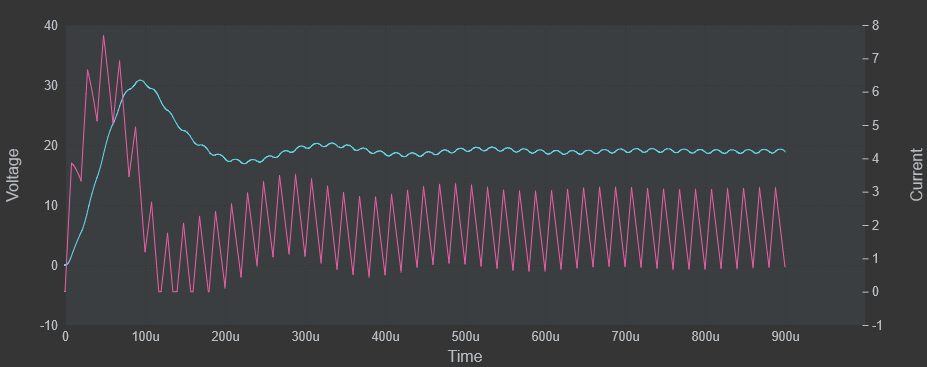
\includegraphics[width=\linewidth]{img/hfd2/IL-Vout.png}
        \caption{\(I_{L}\) and \(V_{out}\)}
        \label{fig:Waveform_IL_Vout}
    \end{subfigure}
    \hfill
    \begin{subfigure}[b]{0.5\linewidth}
        \centering
        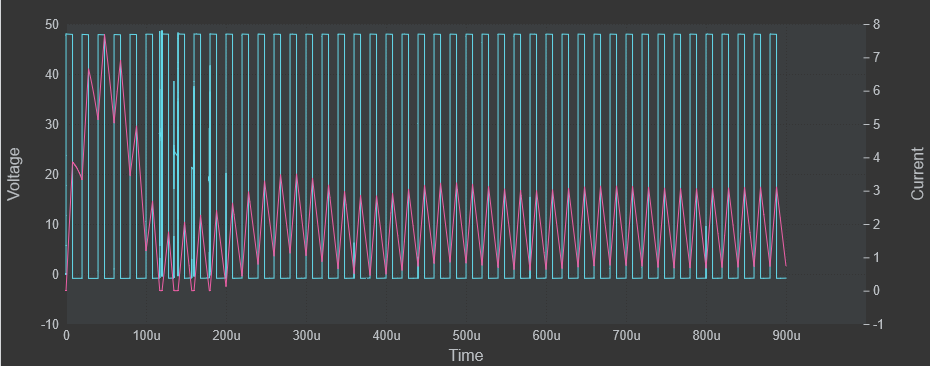
\includegraphics[width=\linewidth]{img/hfd2/IL-Vleg.png}
        \caption{\(I_{L}\) and \(V_{leg}\)}
        \label{fig:Waveform_IL_VLeg}
    \end{subfigure}
    \caption{Waveforms}
    \label{fig:Waveforms}
\end{figure}

Met deze waarden ingevoerd in de simulatie genereren we een reeks golfvormen die de inductorstroom \( I_L \) in relatie tot andere circuitcomponenten illustreren. Figuur \ref{fig:Waveforms} toont de golfvormen van \( I_L \) naast de uitgangsspanning \( V_{out} \) en de spanningspoot \( V_{leg} \). Daarnaast geeft Figuur \ref{fig:Waveforms_IL_all} gedetailleerde vergelijkingen van de golfvormen van \( I_L \) met de drain-source stroom \( I_{DS} \), diodestroom \( I_{D} \), condensatorstroom \( I_{C} \), weerstandsstroom \( I_{R} \), en ingangsstroom \( I_{\text{in}} \). Deze vergelijkingen helpen om de stroomrichting en spanningsniveaus door het circuit heen te visualiseren.

\begin{figure}[h!]
    \centering
    \begin{subfigure}[b]{0.45\linewidth}
        \centering
        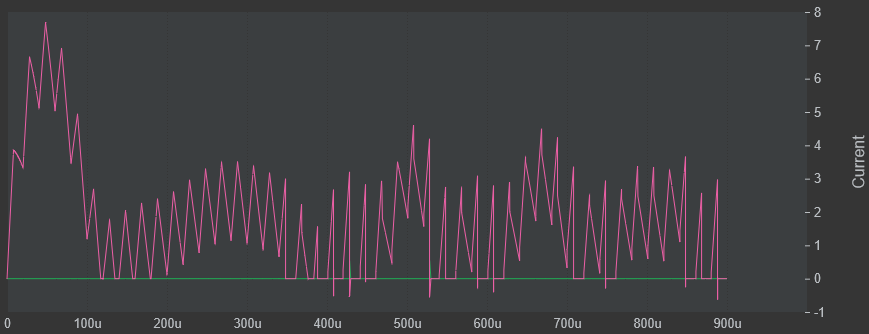
\includegraphics[width=\linewidth]{img/hfd2/IL-IDS.png}
        \caption{Waveform of \(I_{L}\) and \(I_{DS}\)}
        \label{fig:Waveform_IL_IDS}
    \end{subfigure}
    \hfill
    \begin{subfigure}[b]{0.45\linewidth}
        \centering
        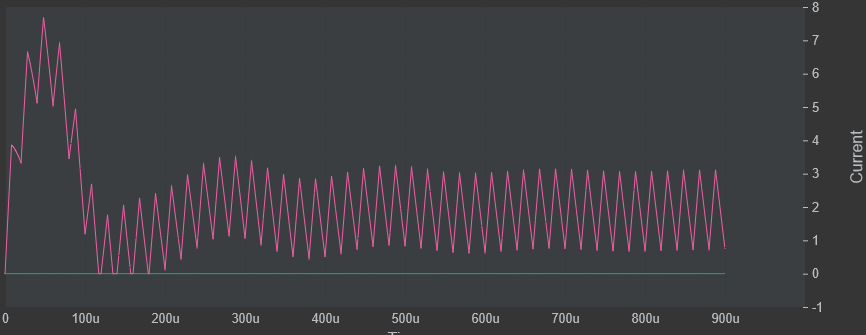
\includegraphics[width=\linewidth]{img/hfd2/IL-ID.png}
        \caption{Waveform of \(I_{L}\) and \(I_{D}\)}
        \label{fig:Waveform_IL_ID}
    \end{subfigure}
    
    \begin{subfigure}[b]{0.45\linewidth}
        \centering
        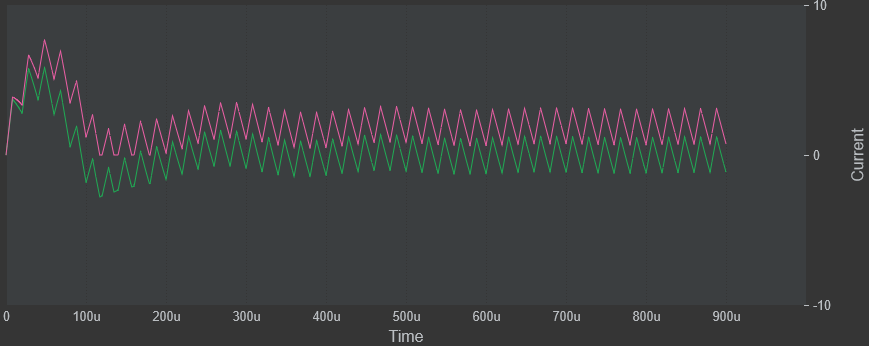
\includegraphics[width=\linewidth]{img/hfd2/IL-IC.png}
        \caption{Waveform of \(I_{L}\) and \(I_{C}\)}
        \label{fig:Waveform_IL_IC}
    \end{subfigure}
    \hfill
    \begin{subfigure}[b]{0.45\linewidth}
        \centering
        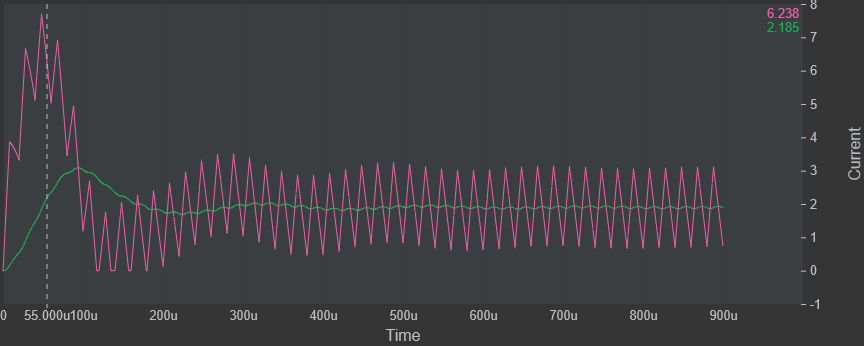
\includegraphics[width=\linewidth]{img/hfd2/IL-IR.png}
        \caption{Waveform of \(I_{L}\) and \(I_{R}\)}
        \label{fig:Waveform_IL_IR}
    \end{subfigure}
    
    \begin{subfigure}[b]{0.45\linewidth}
        \centering
        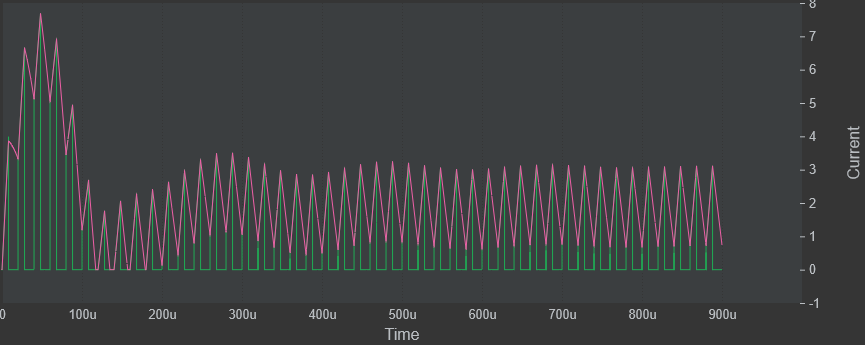
\includegraphics[width=\linewidth]{img/hfd2/IL-Lin.png}
        \caption{Waveform of \(I_{L}\) and \(I_{\text{in}}\)}
        \label{fig:Waveform_IL_Lin}
    \end{subfigure}
    
    \caption{Waveforms comparing \(I_{L}\) with various parameters: \(I_{DS}\), \(I_{D}\), \(I_{C}\), \(I_{R}\), and \(I_{\text{in}}\)}
    \label{fig:Waveforms_IL_all}
\end{figure}

Elke golfvorm biedt inzicht in het schakelgedrag, de energieoverdracht en de verliezen binnen de buck converter onder omstandigheden van continue inductorstroom, wat cruciaal is voor het begrijpen van de efficiëntie en stabiliteit van de converter.
\subsection{Waveforms Buck Converter, discontinuous inductor current}
\phantomsection
\addcontentsline{toc}{section}{Referenties}
\printbibliography
\end{document}
